\documentclass[aspectratio=169,xcolor=dvipsnames]{beamer}
\usepackage[portuguese]{babel}
\usepackage[utf8]{inputenc}
\usepackage{hyperref}
\usepackage{graphicx}
\usepackage{booktabs}
\usepackage{listings}
\usepackage{animate}  

\title[]{Sistema CRUD de Locação de Veículos}
\author{Gabriel Sales Costa \newline Igor Masson Calille \newline Pedro Alcantara Krivochein}
\institute[PUC-SP]{Pontifícia Universidade Católica de São Paulo}
\date{\today}

\setbeamertemplate{footline}[frame number]
\setbeamertemplate{navigation symbols}{}

\lstset{
    language=Python,
    basicstyle=\ttfamily\small,
    breaklines=true,
    keywordstyle=\color{blue},
    stringstyle=\color{red},
    commentstyle=\color{green},
    morecomment=[l][\color{magenta}]{\#}
}

\begin{document}

\frame{\titlepage}

\section{Introdução}
\begin{frame}
\frametitle{Introdução}
\begin{itemize}
    \item Sistema desenvolvido para facilitar a gestão de veículos para locação.
    \item Objetivos:
    \begin{itemize}
        \item Automatizar processos de reserva e devolução.
        \item Melhorar a eficiência operacional.
    \end{itemize}
\end{itemize}
\end{frame}

\section{Visão Geral do Projeto}
\begin{frame}
\frametitle{Visão Geral do Projeto}
\begin{itemize}
    \item O que é um CRUD?
    \begin{itemize}
        \item Create: Adicionar novos registros.
        \item Read: Ler dados existentes.
        \item Update: Atualizar dados existentes.
        \item Delete: Remover registros.
    \end{itemize}
    \item Aplicação do CRUD no sistema de locação de veículos:
    \begin{itemize}
        \item Gerenciamento de clientes.
        \item Controle de veículos.
        \item Processamento de reservas.
    \end{itemize}
\end{itemize}
\end{frame}

\section{DER (Diagrama Entidade-Relacionamento)}
\begin{frame}
\frametitle{DER (Diagrama Entidade-Relacionamento)}
\begin{center}
    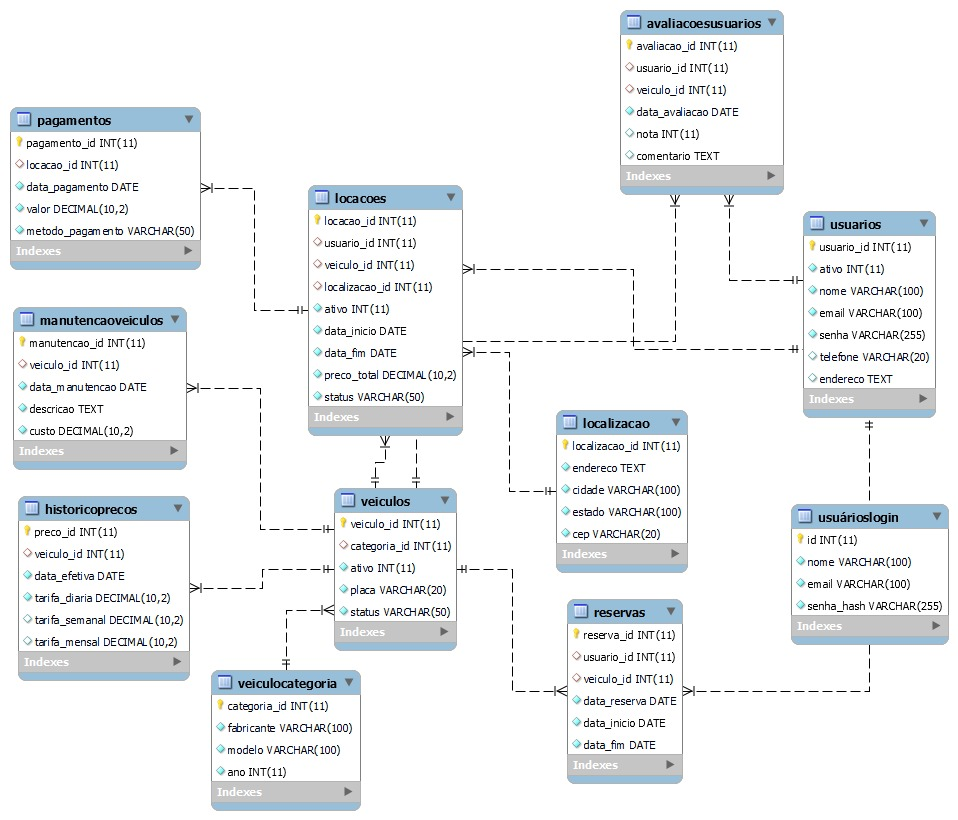
\includegraphics[width=0.65\textwidth]{images/DER.jpg} 
\end{center}
\end{frame}

\section{Tecnologias Utilizadas}
\begin{frame}
\frametitle{Tecnologias Utilizadas}
\begin{itemize}
    \item \textbf{Back-End:}
    \begin{itemize}
        \item Python
        \item Flask
        \item MySQL
    \end{itemize}
    \item \textbf{Front-End:}
    \begin{itemize}
        \item HTML
        \item CSS
        \item JavaScript
    \end{itemize}
\end{itemize}
\end{frame}

\section{Conexão Python-MySQL com Flask}
\begin{frame}[fragile]
\frametitle{Conexão Python-MySQL com Flask}
\begin{itemize}
    \item função de conexão com o banco de dados MySQL.
\end{itemize}
\begin{lstlisting}

# Configurações do banco de dados
db = mysql.connector.connect(
    host="localhost",
    user="usuario",
    password="senha",
    database="locacao_veiculos"
)

\end{lstlisting}
\end{frame}

\section{Operando API com Flask}
\begin{frame}[fragile]
\frametitle{Conexão Python-MySQL com Flask}
\begin{itemize}
    \item Exemplo de função Read para obter o relatório das locações.
\end{itemize}
\begin{lstlisting}

    # Read - Obter todas as locacoes
    @locacoes_bp.route('/', methods=['GET'])
    def read_locacoes():
        connection = get_db_connection()
        cursor = connection.cursor(dictionary=True)
        cursor.execute('SELECT * FROM Locacoes WHERE ativo=1')
        locacoes = cursor.fetchall()
        cursor.close()
        connection.close()
        return render_template('locacoes.html', locacoes=locacoes)
\end{lstlisting}
\end{frame}


\section{Demonstração do Front-End - Login}
\begin{frame}
\frametitle{Demonstração do Front-End - Login}
\begin{itemize}
 \item Tela de login:
\end{itemize}
\begin{figure}
    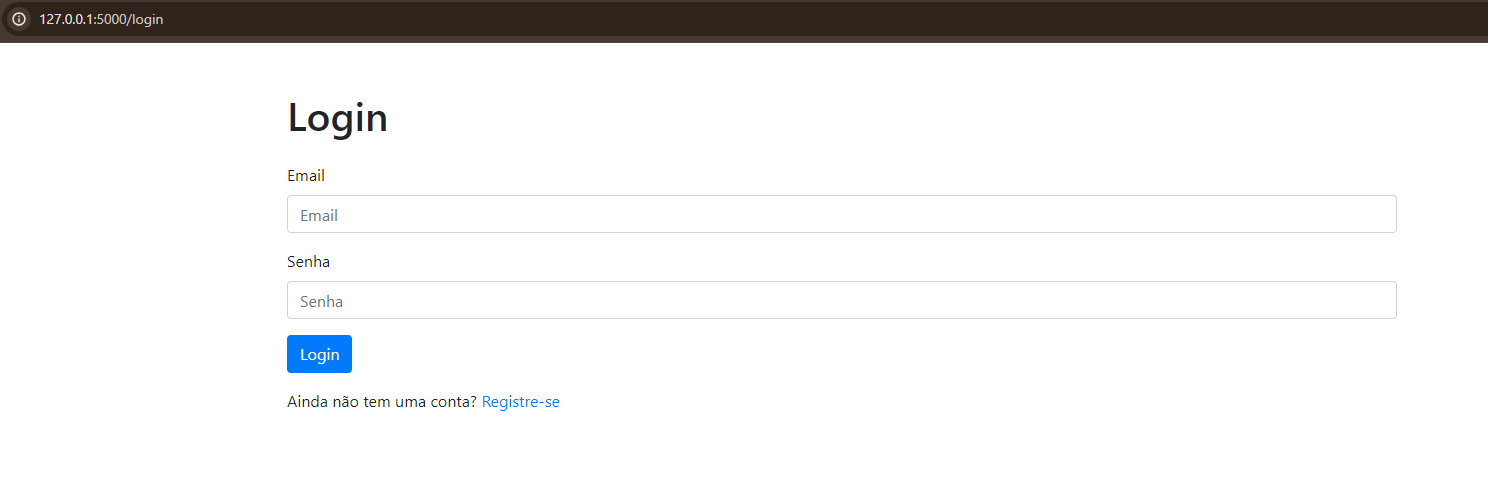
\includegraphics[width=0.80\textwidth]{images/Login.png} 
\end{figure}
\end{frame}

\section{Demonstração do Front-End - Interface CRUD com relatório}
\begin{frame}
\frametitle{Demonstração do Front-End - Interface CRUD com relatório}
\begin{itemize}
 \item Interface:
\end{itemize}
\begin{figure}
    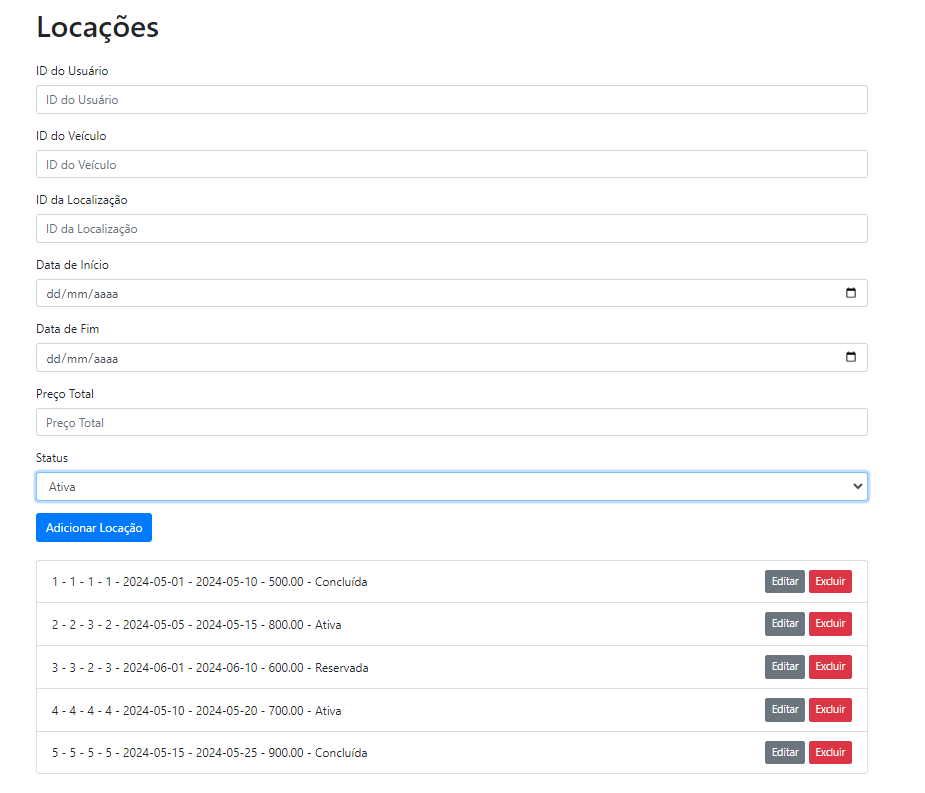
\includegraphics[width=0.60\textwidth]{images/relatorio.png} 
\end{figure}
\end{frame}

\section{Conclusão}
\begin{frame}
\frametitle{Conclusão}
\begin{itemize}
    \item \textbf{Resumo dos principais pontos abordados:}
    \begin{itemize}
        \item Desenvolvimento de um sistema de locação de veículos utilizando a arquitetura CRUD.
        \item Integração de tecnologias como:
        \begin{itemize}
            \item Python e Flask para o desenvolvimento do back-end.
            \item MySQL como banco de dados relacional.
            \item HTML, CSS e JavaScript para a construção de um front-end interativo e responsivo.
        \end{itemize}
        \item Implementação de um Diagrama Entidade-Relacionamento (DER) bem estruturado, que suporta as operações de negócios necessárias.
    \end{itemize}
    \item \textbf{GitHub do Projeto:} \href{https://github.com/Igor-Calille/Python-Projects/tree/main/Sistema-Loca\%C3\%A7\%C3\%A3o-Veiculos}{Sistema de Locação de Veículos}
\end{itemize}
\end{frame}





\begin{frame}
    \Huge{\centerline{Fim}}
\end{frame}

\end{document}
